\chapter{Manuale d'uso}
Affrontiamo ora la parte piu' pratica del progetto.
\section{Installazione}
Anzitutto e' importante sapere che per poter utilizzare il prodotto da noi creato e' necessaria almeno una rete LAN o una rete INTERNET.
Un computer della rete deve fornire il servizio di bootstrap Server e quindi deve essere avviato come tale.
All'avvio del programma l' utente può decidere se essere un SuperNode o un OrdinaryNode.
Ricordiamo che questa decisione non sarà possibile modificarla nel seguito. 
A seconda della scelta appariranno a video le schermate da utilizzare ed il programma è pronto a funzionare.
\section{Primo avvio}
\begin{figure}[t]
 \centering
 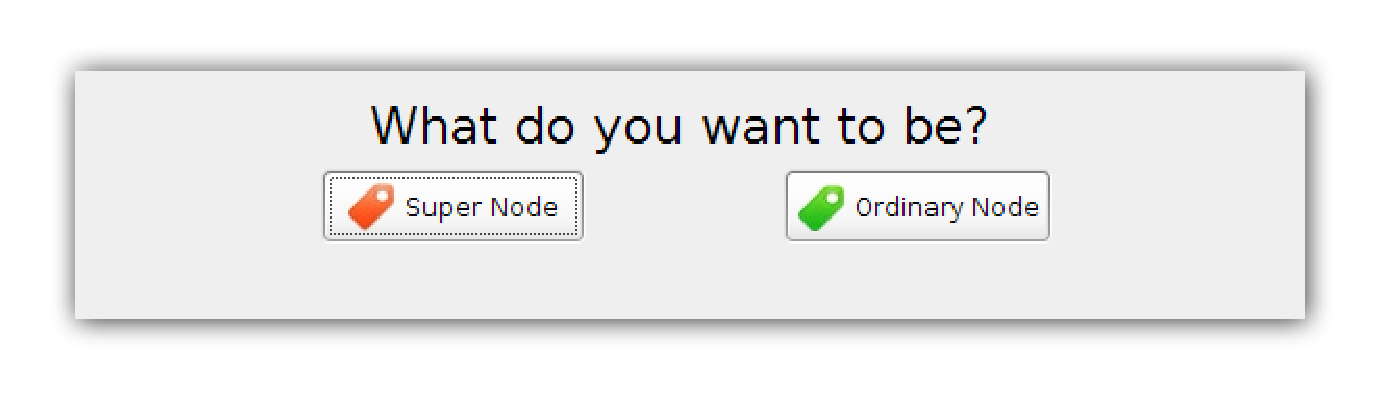
\includegraphics[width=325px,height=75px]{images/what.eps}
 % logica_uml.eps: 0x0 pixel, 300dpi, 0.00x0.00 cm, bb=14 14 593 376
 \caption{Pannello di decisione SuperNode o OrdinaryNode}
 \label{fig:what}
\end{figure}
Per semplicità spieghiamo il primo avvio supponendo di lanciae la nostra applicazione in modalità SuperNode.
Le cose che verranno scritte nella parte sottostante sono analoghe anche se si lanciasse la modalità
OrdinaryNode.
All'avvio appare la schermata mostrata in Figura \ref{fig:what}.
Cliccando sul tasto che corrisponde alla creazione di supernode appare un nuovo pannello mostrato 
in Figura \ref{fig:configuration}.
\begin{figure}[t]
 \centering
 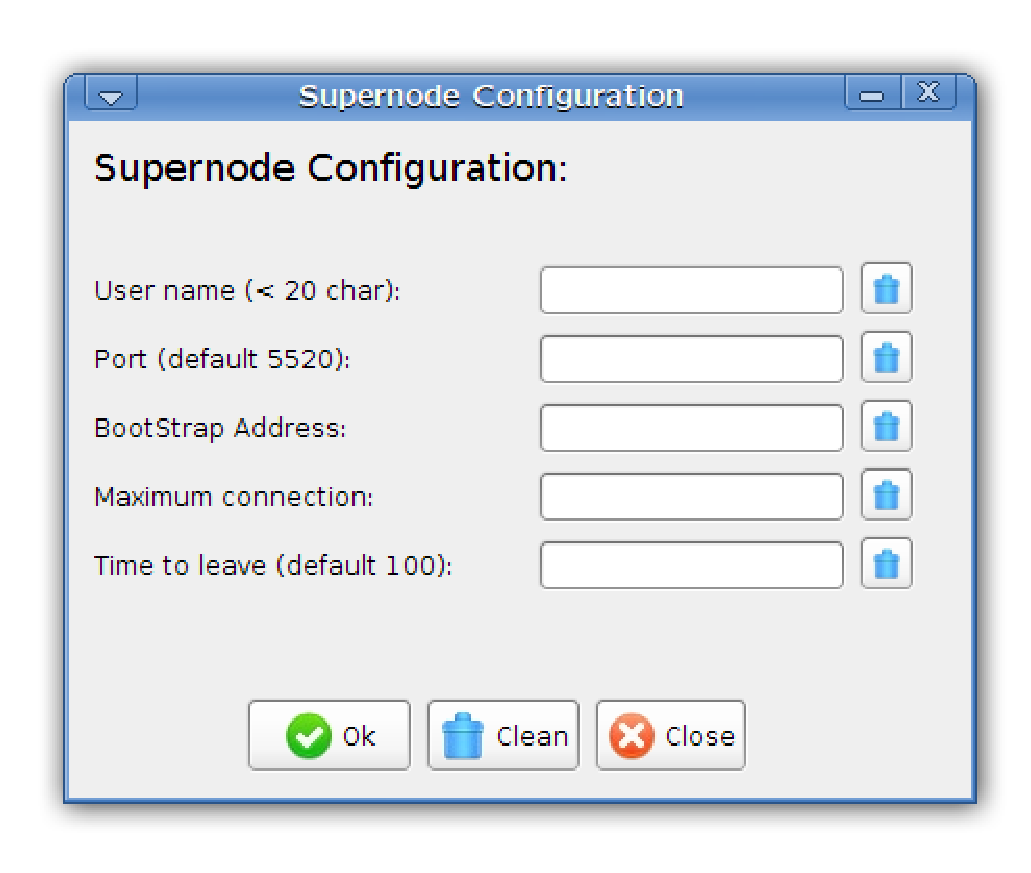
\includegraphics[width=325px,height=200px]{images/configuration.eps}
 % logica_uml.eps: 0x0 pixel, 300dpi, 0.00x0.00 cm, bb=14 14 593 376
 \caption{Il pannello di configurazione del SuperNode.}
 \label{fig:configuration}
\end{figure}
E' necessario ora riempire i campi vuoti per la configurazione del peer.
Inseriamo quindi un nikname che preferiamo, il numero della porta di comunicazione, l' indirizzo del bootstrap server,
il massimo numero di nodi al quale verrà inviata la richiesta di un file ed infine il time to live.
Il settaggio del time to live lo sconsigliamo ad utenti poco esperti dato che potrebbe, se impostato male, rendere l' applicazione
poco funzionante.
Consigliamo inoltre ad utenti esperti che intendano settare il time to live di farlo in modo oculato. 
Per l'applicazione utilizzata su reti di grosse dimensioni è preferibile un time to live maggiore di quello 
impostato di default, mentre al contrario se si lancia l' applicativo su reti di piccola dimensione è preferibile un time to live decisamente 
più piccolo di quello di default.
\begin{figure}[t]
 \centering
 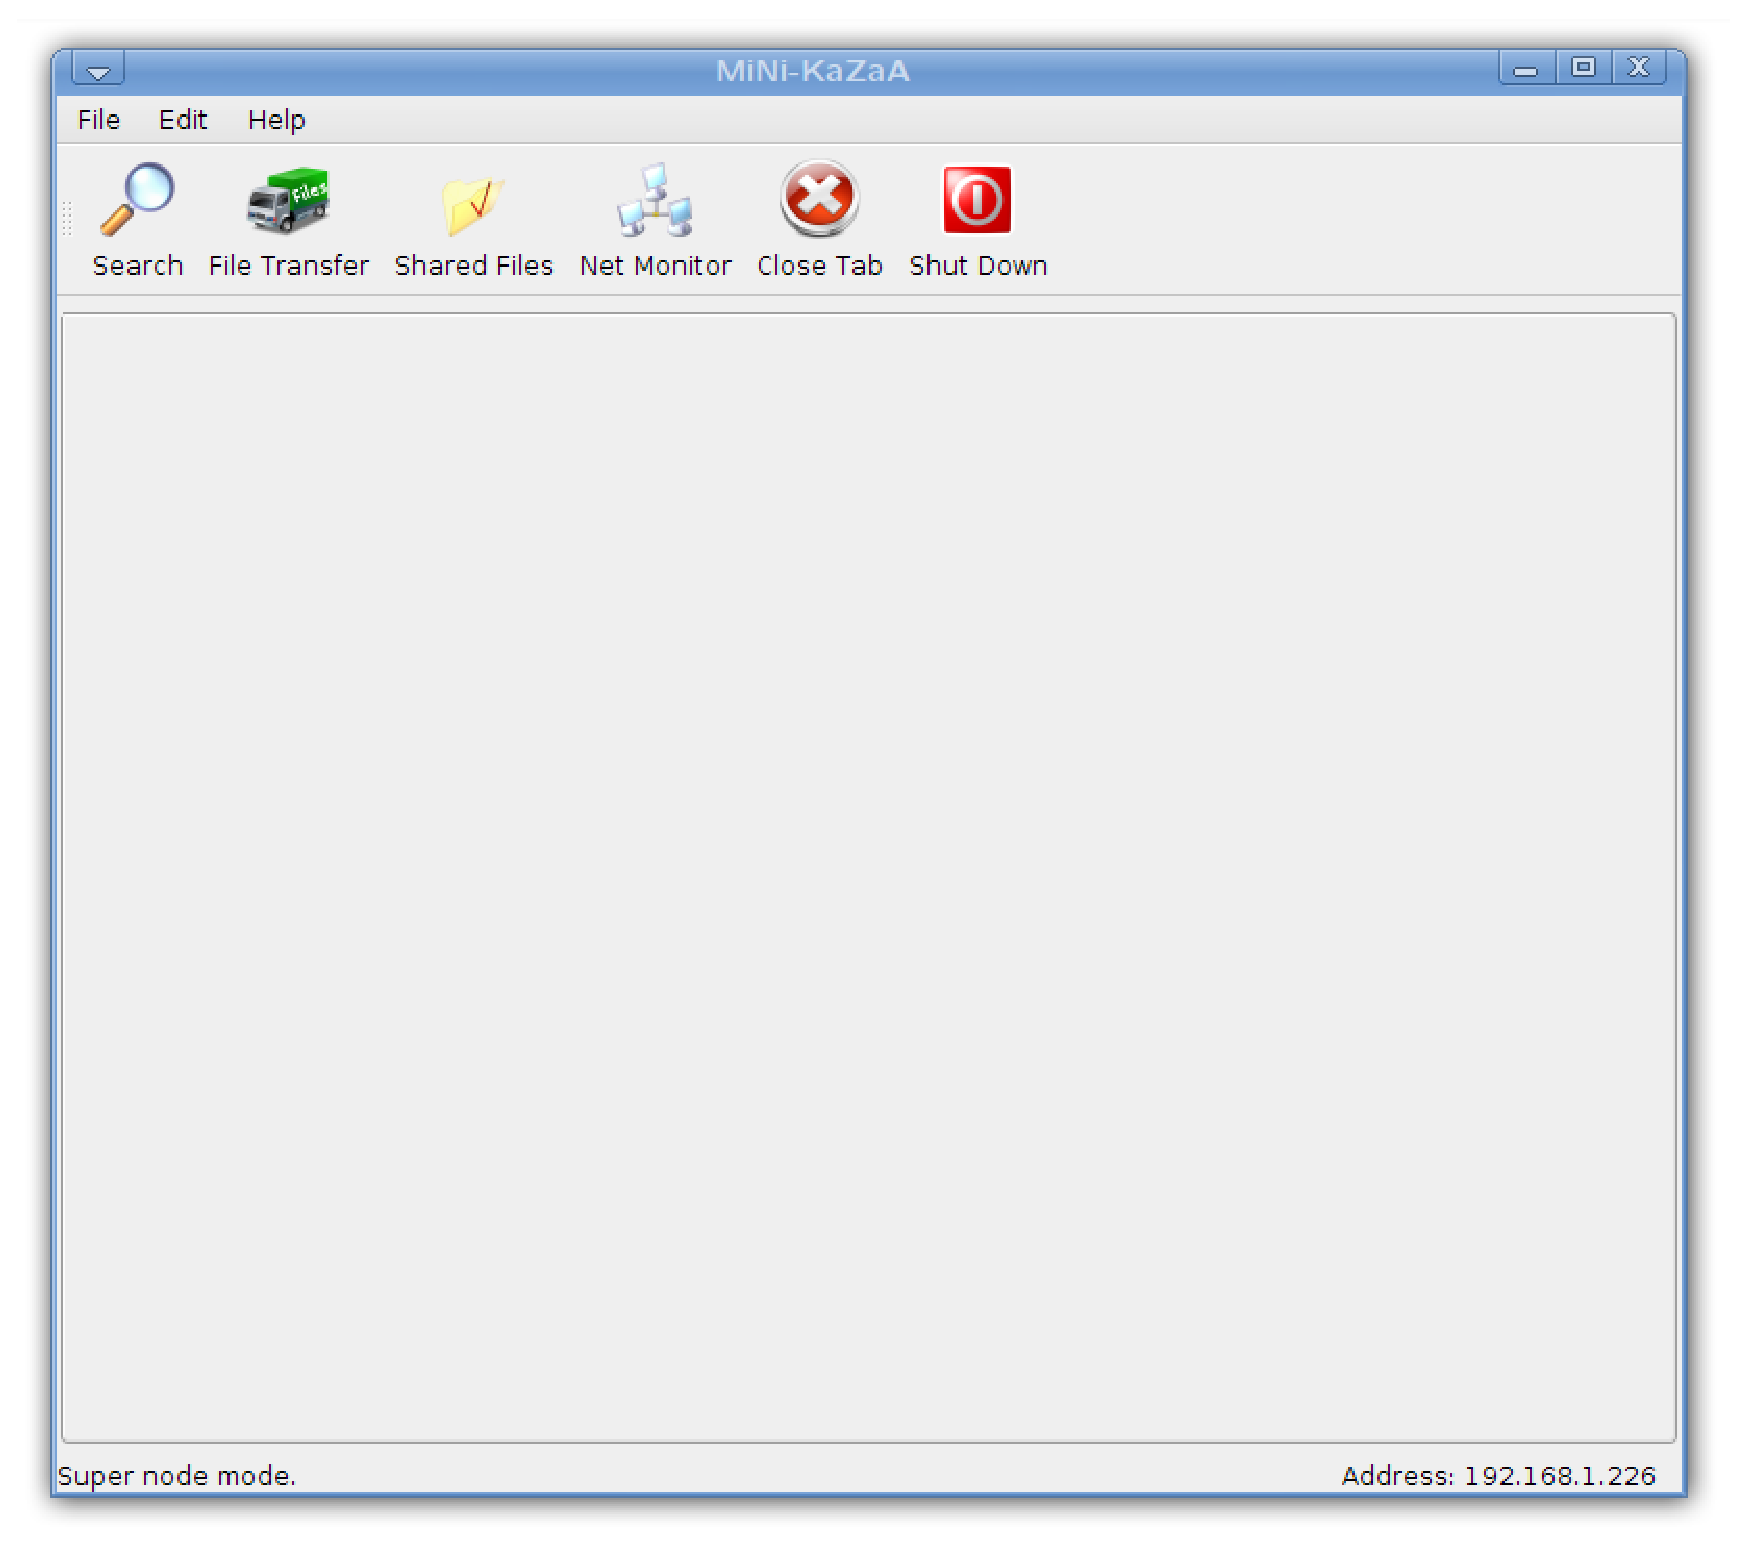
\includegraphics[width=350px,height=225px]{images/mini_kazaa_client.eps}
 % logica_uml.eps: 0x0 pixel, 300dpi, 0.00x0.00 cm, bb=14 14 593 376
 \caption{L' interfaccia principale dell' ordinary node.}
 \label{fig:mini}
\end{figure}
Riempiti tutti i campi correttamente e premuto il tasto ok, se tutto è andato a buon fine apparirà ora la finestra in figura 
\ref{fig:mini}
In caso di campi compilati in maniera non corretta il client provvede a segnalare l'errore con un'apposita \emph{dialog}.
L' installazione è terminata, il programma è funzionanante non vi resta che divertirvi con Mini-KaZaA.

\section{Come funziona}
Bene se siamo di fronte al programma correttamente installato ora non ci rimane che usarlo.
Se abbiamo deciso di essere SuperNode noi vogliamo oltre che poter cercare e scaricare sulla rete fornire il nostro servizio alla comunica globale.
Se abbiamo decido di essere OrdinaryNode noi vogliamo usufruire solamente del servizio di ricerca e download che offre Minikazaa.
	\subsection{Cercare e scaricare un file}
Per cercare e scaricare un file, è necessario inserire nella casella vuota il titolo del file che interessa trovare nella rete.
La nostra casella di ricerca interpreta la parola chiave inserita della casella come una $ *esempio* $ . Questo significa che tutti i file che contengono nel titolo la parola "esempio" verranno restituiti come canditati per lo scaricamento.
Nella tabellina sotto il campo dove è stata inserita la parola ora appariranno i riferimenti ai file che sono presenti sulla rete, i quali possono essere facilmente scaricati cliccando su comodo pulsate download
Il download che parte automaticamente è visibile e controllabile nella sezione chiamata FILETRANSFERT.

	\subsection{Aggiungere un file nella lista dei file condivisi}
Come tutti i servizi di file sharing minikazaa permette di aggiornare la lista dei file che è possibile scaricare.
Cliccando il bottone di Sharing viene caricato automaticamente un pannello che indica la lista dei file che sono stati messi in condivisione nella rete.
E' inoltre possibile aggiungere file alla lista cliccando su tasto add e rimuoverne altri cliccando sul tasto remove.

	\subsection{Controllare lo stato dei download}
Cliccando la sezione FileTranfert si apre un pannello che permette di controllare lo stato dei download dei file che desideriamo scaricare.
Nella tabella che si è appena aperta è possibile vedere il nome del file, la dimensione e il progressivo stato di scaricamento nella barra.

	\subsection{NetMonitor}
Questo tasto risulta disabilitato se avete deciso di essere OrdinaryNode e invece è attivo se avete deciso di essere SuperNode.
Prendiamo ora il caso di essere SuperNode, e di avere aperto il pannello corrispondente a NetMonitor.
Nel suddetto pannello appare la situazione della rete al momento, piu' precisamente la lista dei SuperNode ai quali si è connessi.


	\subsection{Chiudere le schede}
I restanti tasti visibili nella schermata permettono di chiudere le schede aperte in precedenza.

	\section{Consigli degli autori per l' utilizzo}
Al fine di rendere un migliore servizio possibile diamo alcuni consigli per gli utilizzatori del nostro software.
Consigliamo quindi ad utilizzatori dotati di grosse quantità di file, ma soprattutto di grandi capacità di linea di offrire il loro servizio alla comunità globale e quindi di avviare l' applicazione come supernode.
Consigliamo invece agli utenti di piccole dimensione, che hanno difficolta ed un valore di upload limitato di preferire la modalità da ordinaryNode.
  
